\begin{figure}[h]
\begin{center}
	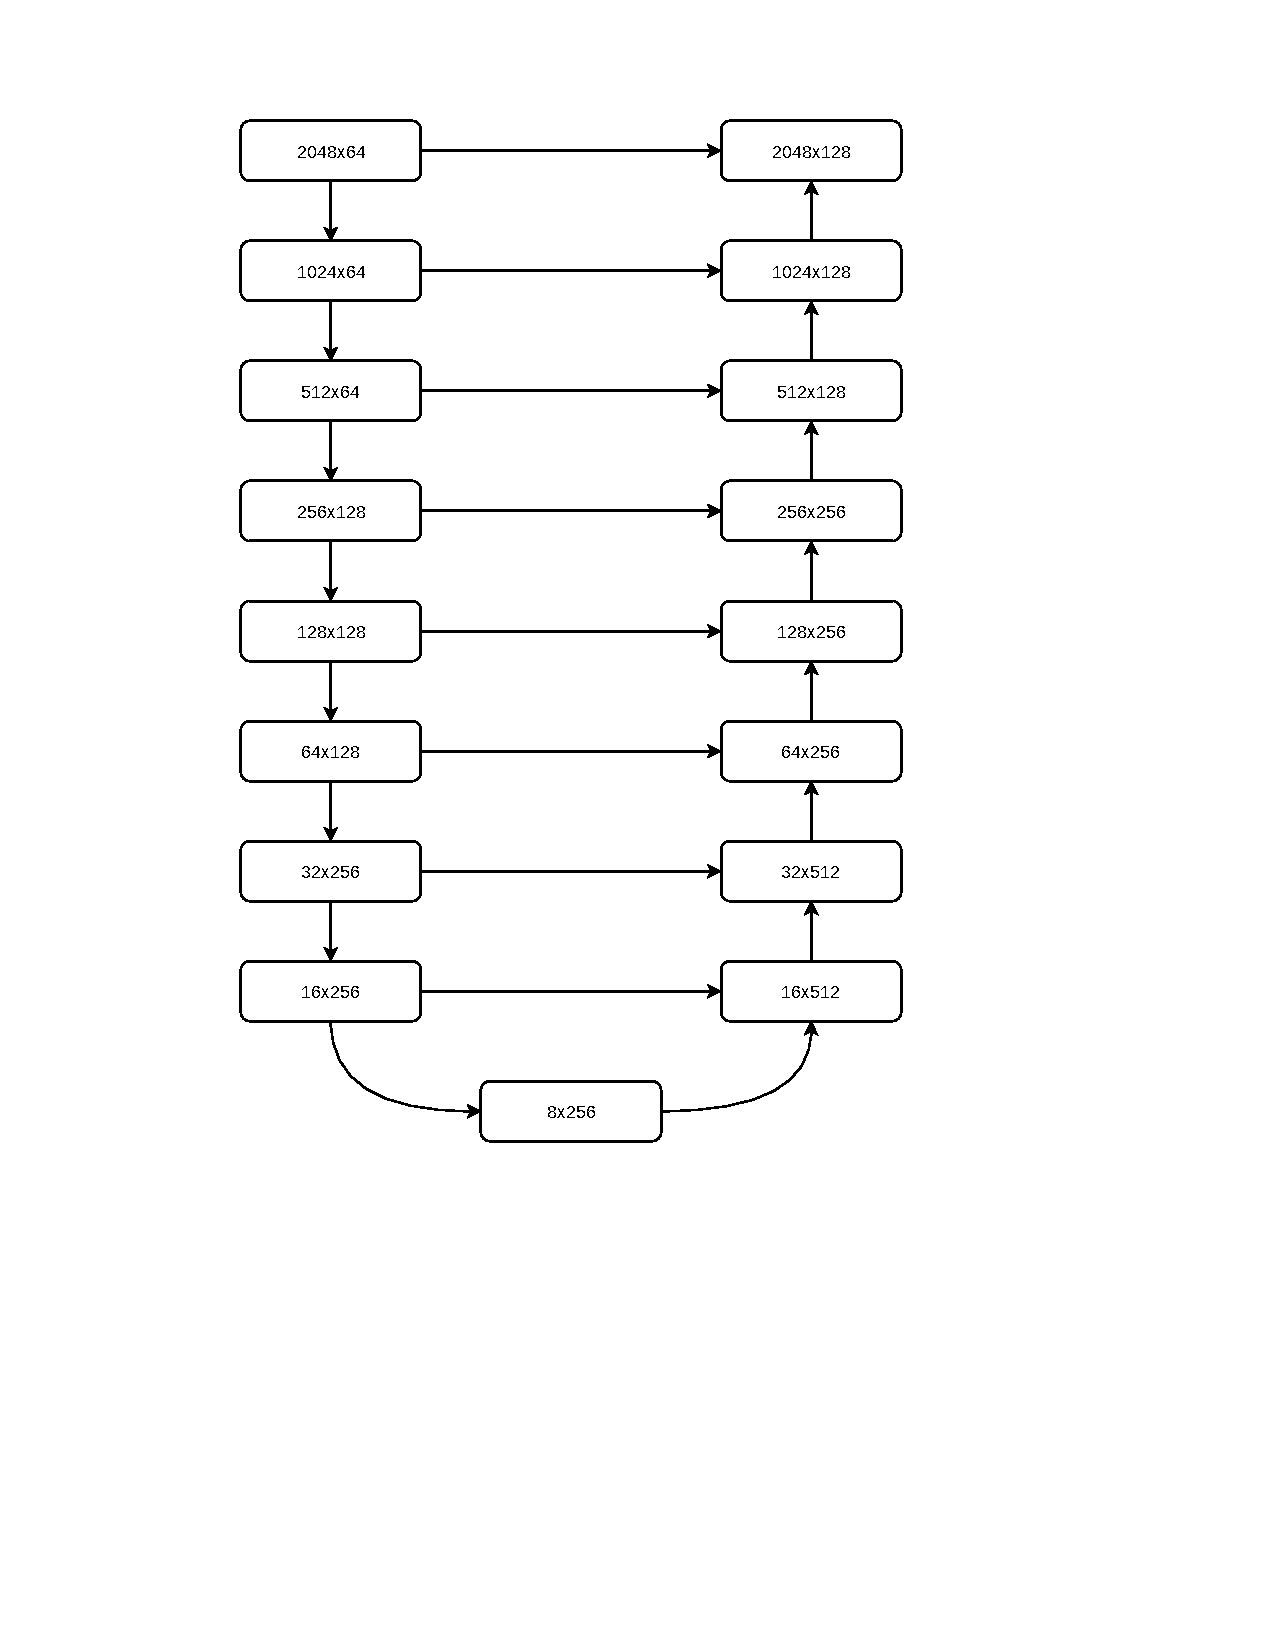
\includegraphics[width=0.5\textwidth]{architecture}
	\caption{Model Architecture}
	\label{fig:architecture}
\end{center}
\end{figure}

\noindent The two networks used are both based on the U-Net architecture originally proposed for speech enhancement/denoising in \cite{pandey_new_2019}. The specific layer sizes and the architecture of each block is detailed in figure \ref{fig:architecture}. The time-domain network replaces the final rectified linear unit activation with a hyperbolic tangent activation to produce values between -1 and 1. The frequency domain network is one block in a larger traditional signal processing system shown in figure \ref{fig:systems}.

\begin{figure}[h]
	\centering
	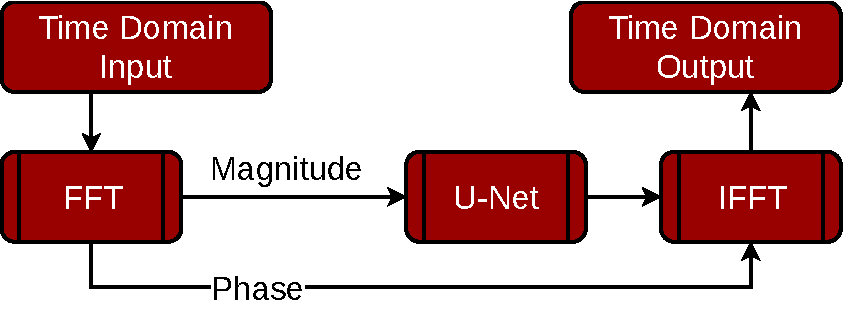
\includegraphics[width=0.5\textwidth]{systems_2}
	\caption{System Architecture of Frequency domain Network}
	\label{fig:systems}
\end{figure}

